\documentclass{article}

% if you need to pass options to natbib, use, e.g.:
% \PassOptionsToPackage{numbers, compress}{natbib}
% before loading nips_2017
%
% to avoid loading the natbib package, add option nonatbib:
% \usepackage[nonatbib]{nips_2017}

\usepackage[final]{nips_2017}

% to compile a camera-ready version, add the [final] option, e.g.:
% \usepackage[final]{nips_2017}

\usepackage[utf8]{inputenc} % allow utf-8 input
\usepackage[T1]{fontenc}    % use 8-bit T1 fonts
\usepackage{hyperref}       % hyperlinks
\usepackage{url}            % simple URL typesetting
\usepackage{booktabs}       % professional-quality tables
\usepackage{amsfonts}       % blackboard math symbols
\usepackage{nicefrac}       % compact symbols for 1/2, etc.
\usepackage{microtype}      % microtypography
\usepackage{graphicx}
\usepackage{natbib}

\graphicspath{{figures/}}

\title{Cracking Neural Network Hashes with Adversarial Examples}

% The \author macro works with any number of authors. There are two
% commands used to separate the names and addresses of multiple
% authors: \And and \AND.
%
% Using \And between authors leaves it to LaTeX to determine where to
% break the lines. Using \AND forces a line break at that point. So,
% if LaTeX puts 3 of 4 authors names on the first line, and the last
% on the second line, try using \AND instead of \And before the third
% author name.

\author{
  Conrad ~Christensen\\
  Deep Learning, Spring 2018\\
  New York University\\
  \href{mailto:conradbc@cims.nyu.edu}{\texttt{conradbc@cims.nyu.edu}} \\
  \And
  Da ~Ying\\
  Deep Learning, Spring 2018\\
  New York University\\
  \href{mailto:dy877@nyu.edu}{\texttt{dy877@nyu.edu}}
}

\begin{document}
% \nipsfinalcopy is no longer used

\maketitle

\begin{abstract}
    Success of neural networks have lead to a wide range of applications, some
    more appropriate than others. Due to a potential for parallelization, and
    ease of implementation, some works have suggested using neural networks as
    hash functions.  We believe this is a bad idea in terms of security, as
    neural networks are differentiable, which allows methods for collision
    search. We show that it is possible to generate hash collisions for some of
    the basic neural network hash functions. Additionally we explore the
    applicability of multiple techniques from adversarial example generation on
    generating collisions for a neural network hashing algorithm, comparing
    their efficacy.
\end{abstract}

\section{Introduction}

\section{Related Work}

The two areas of literature that concern our project are \emph{adversarial examples},
and \emph{Neural hash functions}.

Interest in adversarial examples started around the time of their description
in \cite{intriguing}. Here authors discovered that it is possible to craft
example images that look very much like one class, yet are confidently classified
as another by a neural network.

After this result, Goodfellow et. al. developed a faster method of generating
adversarial examples and studied some of their properties in \cite{explaining}.
One of the original thoughts as to the reason for these was due to un-smooth 
loss surfaces, which led to a proposed defense though distillation \cite{distil}.

Though distillation seemed promising, it turned out it was only performing well
on simple attacks. In fact, adversarial examples were shown to be relatively
robust, living in about 25 dimensions of the input data space \cite{space}.

Many attacks using adversarial examples have been performed on RL policies, vision,
and audio \cite{policy,intriguing,audio}. There have also been numerous techniques
for defense against these attacks, some based on robust optimization, and others
on ensemble models \cite{robust,ensemble}.

Because the model for neural network hashing is known, same model and parameters can be used for white box attacks. To generate hash collisions, targeted attacks are needed so that outputs will match random existing hashes in the dataset. 


Neural network popularity has led to many unique uses for them. Some in already
solved domains. In \cite{hash1} an RNN is used to process data and produce
a fixed length hash value. This work measured the entropy of the hash function
by how many digits in the hash hexadecimal code were changed. Other authors,
including \cite{hash2} have also proposed using neural networks to create
one-way hash functions.

\section{Neural Hash Function}

%%% Separate image locations
%\begin{figure}[t]
    %\centering
    %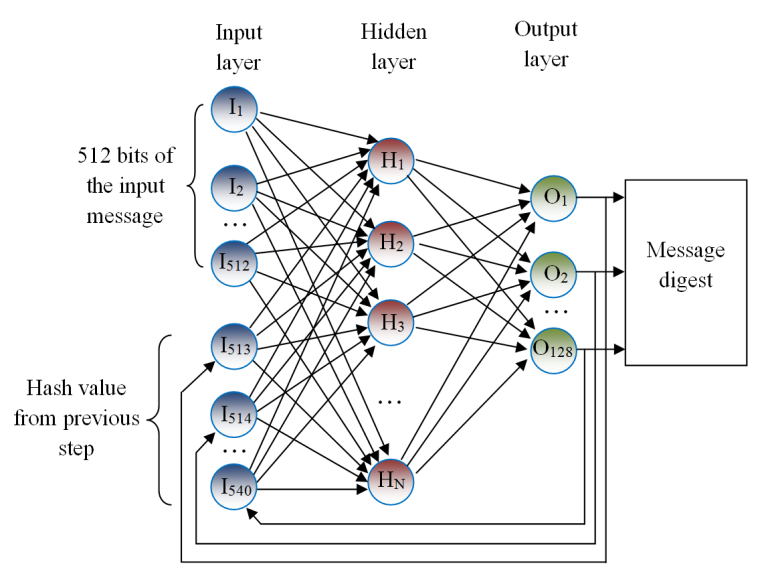
\includegraphics[width=90mm]{hash_nn_architecture}
    %\caption{A simple caption} 
    %\label{fig:hashNN}
%\end{figure}

%\begin{figure}[b]
    %\centering
    %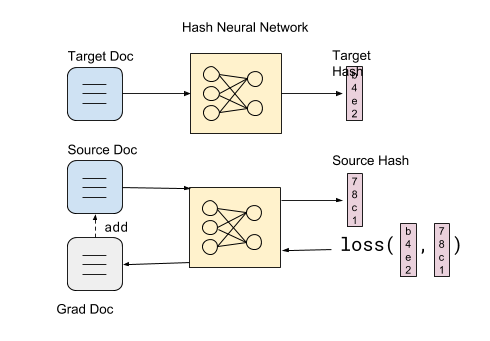
\includegraphics[width=90mm]{model_diagram}
    %\caption{Collision attack overview} 
    %\label{fig:model}
%\end{figure}


%%% Images side-by-side with minipages to save room.
\begin{figure}[t]
    \centering
    \begin{minipage}{.5\textwidth}
        \centering
        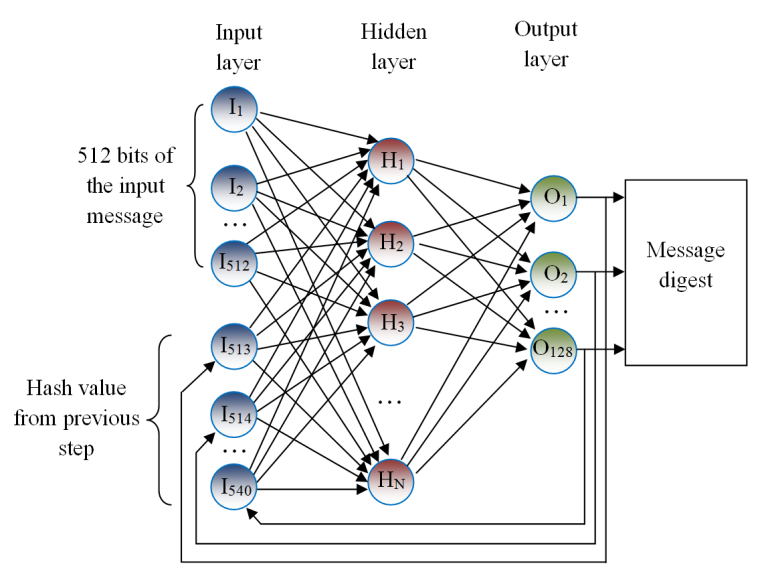
\includegraphics[width=\textwidth]{hash_nn_architecture}
        \caption{Hash function algorithm presented in \cite{hash1}}
        \label{fig:hashNN}
    \end{minipage}%
    \begin{minipage}{.5\textwidth}
        \centering
        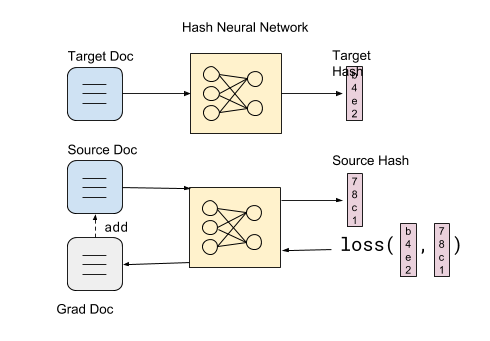
\includegraphics[width=\textwidth]{model_diagram}
        \caption{Collision attack overview} 
        \label{fig:model}
    \end{minipage}
\end{figure}



Look at the nn hash figure in Figure \ref{fig:hashNN}.

\section{Attack Approach}

Look at image in Figure \ref{fig:model}.

\section{Results}

\section{Conclusion}

\bibliographystyle{unsrt}
\bibliography{ref} 

\end{document}
